%Theorem 5.3 (vgl. Theorem 3.1 in \textcite{aktuellesPaper}, basierend auf \textcite{jordan})
%Theorem 5.3 (vgl. \parencite[Theorem 3.1]{aktuellesPaper}; Jordan et al., 2022)
%Warum Brauchen wir Schärfe und Kalibrieung warum nicht kalibibireung allein
\part{Theoretischer Teil}


\chapter{Grundlagen} \label{chap:Grundlagen}
Für das Verständnis dieses und der folgenden Kapitel werden grundlegende Kenntnisse der Wahrscheinlichkeitstheorie vorausgesetzt. Insbesondere sollten die Begriffe von Zufallsvariablen, Verteilungen, Verteilungsfunktionen, Erwartungswerten und bedingten Wahrscheinlichkeiten bekannt sein. Weiter verwenden wir zudem teilweise eher maßtheoretische Konzepte wie $\sigma$-Algebren oder Markovkerne.

Als allgemeines Nachschlagewerk zur Wahrscheinlichkeitstheorie eignet sich
\textcite{klenke2020wahrscheinlichkeitstheorie}. Für eine übersichtliche aber trotzdem formale
Darstellung der Grundlagen von Wahrscheinlichkeitsräumen kann das erste Kapitel des Vorlesungsskripts von \textcite{vanHandel2007} herangezogen werden. \textcite{grimmett2020probability} bietet ebenfalls eine umfassende
Einführung in die Wahrscheinlichkeitstheorie. Ergänzend werden die für die weiteren Ausführungen relevanten, stärker maßtheoretisch geprägten Begriffe Markovkern und „fast sicher“ in Appendix \ref{seq:stoch_explain} grundlegend erläutert.


In diesem Kapitel führen wir in Abschnitt \ref{seq:perd_space} den theoretischen Rahmen für die Betrachtung probabilistischer Vorhersagen ein. Dazu definieren wir den Vorhersageraum als eine mathematische Struktur, die eine Vorhersagesituation und die darin enthaltenen relevanten Größen formalisiert. Die grundlegende Perspektive besteht darin, sowohl die probabilistische Vorhersage als auch den Vorhersagegegenstand als Zufallsgrößen zu verstehen. Alle folgenden Aspekte der Evaluation probabilistischer Vorhersagen, die wir hier betrachten beruhen auf diesem Grundgedanken. Anschließend stellen wir in Abschnitt \ref{seq:cal_sharp} mit Kalibrierung, Schärfe und Scores die zentralen Aspekte zur Evaluation probabilistischer Vorhersagen vor.

\section{Vorhersageraum} \label{seq:perd_space}
Wir definieren den Vorhersageraum orientiert an \textcite[Definition 2.1]{strahl2017cross} und beschreiben darin die für eine probabilistische Vorhersagesituation relevanten Zufallsgrößen.

\begin{defi}[Vorhersageraum] \label{def::room}
Sei $(\Omega, \mathcal{A}, \mathbb{P})$ ein Wahrscheinlichkeitsraum und $\mathcal{A}_0 \subseteq \mathcal{A}$ eine $\sigma$-Algebra.
Ein \emph{Vorhersageraum} ist ein Tupel $(F, Y)$ mit:
\begin{itemize}
    \item $Y: \Omega \to \R$ ist eine Zufallsvariable auf $\WR$.
    \item $F: \Omega \times \BO \to [0,1]$ ist ein Markovkern von $(\Omega, \mathcal{A}_0)$ nach $(\R, \BO)$.
\end{itemize}{}
\end{defi}

\noindent
$Y$ ist nach dieser Definition der Vorhersagegegenstand, während $F$ die Vorhersage bzw. Vorhersageverteilung beschreibt. Dabei ist die Vorhersage selbst zufällig, also eine zufällige bedingte Verteilungsfunktion: Je nachdem, welches Ereignis $\omega \in \Omega$ eintritt, sind unterschiedliche Vorhersageverteilungen möglich.

Die $\sigma$-Algebra $\mathcal{A}_0$ nennen wir die Informationsmenge der Vorhersage. Sie beschreibt die zur Erstellung der Vorhersage verfügbare Information. 

Im Folgenden identifizieren wir die Vorhersage $F$ über ihre Verteilungsfunktion und schreiben
$F(\omega,y) \coloneqq F(\omega,(-\infty,y]), \;\;y \in \mathbb{R}$. Der Einfachheit halber lassen wir das Argument $\omega$ häufig weg und schreiben  $F \coloneqq F(\omega,\cdot)$. Entsprechend schreiben wir auch $F(y)\coloneqq F(\omega,y)$. Das folgende Beispiel soll das Setting verdeutlichen.

\begin{bsp}[Vorhersageraum]\label{bsp::Room}
Wir wollen die Temperatur in Celsius für morgen vorhersagen. Als Information sind zwei unterschiedliche Punktvorhersagen von heute (d.h. $24$ Stunden vor dem Zielzeitpunkt) gegeben. Diese dienen als Grundlage für eine probabilistische Vorhersage.

Wir übersetzen dieses Szenario jetzt in die Schreibweise des Vorhersageraums aus Definition \ref{def::room}. Zunächst wollen wir den Ereignisraum definieren.

\begin{itemize}
    \item Sei $\omega_1 \coloneqq$ wahre Temperatur morgen, $\omega_2 \coloneqq  \text{Punktvorhersage}_1$ , $\omega_3 \coloneqq \text{Punkt\-vorhersage}_2$
    \item Ein Elementarereignis beschreiben wir als das Tupel $\omega = (\omega_1, \omega_2, \omega_3)$. Es entspricht einer möglichen gemeinsamen Realisation der wahren Temperatur zum Zielzeitpunkt sowie der beiden am Vortag erstellten Punktvorhersagen.
    \item Den \emph{Ereignisraum} können wir entsprechend folgendermaßen aufschreiben: 
    \[
    \Omega \subseteq [-273.15\C \;, \infty) \times [-273.15\C \; ,\infty) \times [-273.15\C \; ,\infty) \subseteq \R^3,
    \] 
    wobei wir im Folgenden der Einfachheit halber die Einheit weglassen.
    \item Der Vorhersagegegenstand $Y$ ist damit die Projektion einer Realisation $\omega$ auf dessen erste Komponente
    \[
    Y: \Omega \to \R, \quad \omega \mapsto \omega_1. 
    \]
    \item Als nächstes wollen wir die probabilistische Vorhersage erzeugen. Dazu stehen uns die zwei Punktvorhersagen zur Verfügung. Die Informationsmenge ist damit die durch diese Punktvorhersagen erzeugte $\sigma$-Algebra. D.h.
    \[
    \mathcal A_0=\sigma(\omega_1,\omega_2).
    \]
    Die wahre Temperatur $\omega_1$ ist zum Vorhersagezeitpunkt unbekannt und geht daher nicht als Information in die Vorhersage ein; andernfalls wäre die Vorhersage trivial, weil der Vorhersagegegenstand bereits bekannt wäre.
    \item Nun spezifizieren wir die Vorhersage. Für dieses Beispiel (andere Vorhersagen sind denkbar) modellieren wir die Temperatur als eine normalverteilte Zufallsvariable mit konstanter Varianz von $2$. Den Erwartungswert der Normalverteilung bestimmen wir durch den Mittelwert der beiden Punktvorhersagen. Damit ist die probabilistische Vorhersage 
    \[
    F:\Omega\times\mathcal B(\mathbb R)\to[0,1]
    \] 
    gegeben durch 
    \[
    F(\omega,\cdot)=\mathcal{N} \Big(\tfrac12(\omega_2+\omega_3),2\Big),
    \]
    wobei wir mit $\mathcal{N}(\mu,\sigma^2)$ eine Normalverteilung mit Mittelwert $\mu$ und Varianz $\sigma^2$ bezeichnen.
    \item Die Information, die diese Vorhersage tatsächlich verwendet, ist die lineare Kombination $\omega_2+\omega_3$. Daher gilt
    \[
    \sigma(F)=\sigma(\omega_2+\omega_3)\subseteq \mathcal{A}_0,
    \]
    wobei $\sigma(F)$ die erzeugte $\sigma$-Algebra durch den Markovkern $F$ beschreibt. Genauer handelt es sich dabei um die kleinste $\sigma$-Algebra sodass die Abbildung $\omega \mapsto F(\omega,x)$ für alle $x \in \mathbb{Q}$ messbar ist \parencite{strahl2017cross}. In diesem Beispiel nutzt die Vorhersage also nicht die gesamte verfügbare Information aus $\mathcal A_0$.
\end{itemize}
 
\end{bsp}{}

\noindent
Empirisch betrachten wir Vorhersage-Beobachtungspaare der Form
\begin{equation}\label{eq:stich}
    (F_1,y_1),\dotsc,(F_n,y_n).
\end{equation}Wir interpretieren diese als Stichproben der gemeinsamen Verteilung von $(F,Y)$ unter dem Wahrscheinlichkeitsmaß $\PW$ des Vorhersageraums \parencite{gneiting2023regression}.
Formal lässt sich diese Sichtweise durch eine Repräsentation auf Basis des zugrundeliegenden Wahrscheinlichkeitsraums $(\Omega, \mathcal{A}, \mathbb{P})$  präzisieren. Auf Ebene der Realisationen $\omega^{(i)} \in \Omega$ schreiben wir
\[
(F_i,y_i)
=\bigl(F(\omega^{(i)},\cdot),Y(\omega^{(i)})\bigr),\qquad i=1,\dotsc,n,
\]
wobei wir die $\omega^{(i)}$ als Realisationen unter $\PW$ verstehen. 

Damit legen wir jedoch lediglich die Marginalverteilung der Stichproben fest. Das heißt, wir behandeln die Tupel so, als stammten sie aus derselben Verteilung, ohne ihre gemeinsame Verteilung vollständig zu spezifizieren. Insbesondere werden keine Unabhängigkeitsannahmen getroffen; Abhängigkeiten zwischen den Paaren bleiben im gewissen Rahmen erlaubt, sind aber unmodelliert.

Für Temperaturvorhersagen hingegen werden Vorhersage-Beobachtungspaare typischerweise aus Messungen zu verschiedenen Zeitpunkten und an unterschiedlichen Orten (z.B. Messstationen) gewonnen \parencite{gneiting2014calibration, vannitsem_statistical_2021}. Dabei liegen häufig räumliche und zeitliche Dynamiken vor. In unserem Vorhersageraum-Setting werden diese Strukturen jedoch nicht explizit modelliert. Das ist insofern vertretbar, weil sich die Bewertung von Vorhersagen primär auf das Zusammenspiel von Vorhersage und Beobachtung konzentriert, nicht auf den gesamten Datenentstehungsprozess. Für Kalibrierung ist es daher nicht unbedingt notwendig, räumliche oder zeitliche Abhängigkeiten der Daten vollständig zu modellieren. Kalibrierung ist hiernach zunächst eine Eigenschaft der gemeinsamen Verteilung  $(F,Y)$. Abhängigkeitsstrukturen können dennoch wichtig sein, z.B. Autokorrelationen von Vorhersagefehlern. Entsprechend gibt es andere Konzeptionen von Vorhersageräumen, die etwa serielle Abhängigkeiten explizit berücksichtigen. Siehe hierzu etwa \textcite[Definition 2.2]{strahl2017cross}. 

Allgemein sowie in dieser Arbeit beschränken wir uns praktisch meistens nur auf die gemeinsame Verteilung von $(F,Y)$, ohne weitere Aspekte der zugrunde liegenden stochastischen Struktur explizit zu modellieren \parencite{gneitingCombining2013}. Liegen mehrere verschiedene Vorhersagen vor, können wir den Vorhersageraum um diese als zusätzliche Markovkerne erweitern.


\begin{bsp}[Stichprobe aus dem Vorhersageraum]
Wir betrachten den Vorhersageraum aus Beispiel \ref{bsp::Room}. Unter einem impliziten Wahrscheinlichkeitsmodell $\PW$ im Vorhersageraum kann eine Stichprobe aus $\omega^{(1)}, \omega^{(2)}, \omega^{(3)} \in \Omega \;$ mit $\;\omega^{(i)} = (\omega_1^{(i)}, \omega_2^{(i)}, \omega_3^{(i)}),\; i \in \{1,2,3\},$ folgendermaßen aussehen:
\[
\omega^{(1)} = (20\C, 17\C, 21\C), 
\;\omega^{(2)} = (25\C, 22\C, 24\C),
\;\omega^{(3)} = (17\C, 17\C, 18\C).
\]
Diese Stichprobe aus Temperaturmessung und Punktvorhersagen könnte beispielsweise an drei verschieden Tagen oder Orten entstanden sein. Daraus ergeben sich für die Vorhersage-Beobachtungspaare
\[
(F_i,y_i) \quad  \text{mit} \quad F_i=F(\omega^{(i)},\cdot)  \quad \text{und} \quad y_i = Y(\omega^{(i)})= \omega_1^{(i)}
\]
folgende Werte
\[
\left(\N\left(19,2\right),20\right),
\left(\N(23,2),25\right),
\left(\N(17.5\;,2),17\right). 
\]
Diese Vorhersage-Beobachtungspaare können wir nun nutzen, um die Güte der Vorhersage zu bewerten.
\end{bsp}{}


\section{Kalibrierung und Schärfe} \label{seq:cal_sharp}
Wollen wir probabilistische Vorhersagen beurteilen, so sind nach \textcite{gneiting2014probabilistic} zwei wichtige Eigenschaften zu beachten: Kalibrierung und Schärfe der Vorhersage. Kalibrierung beschreibt, inwieweit die vorhergesagten Verteilungen der tatsächlichen Verteilung des Vorhersagegegenstandes entspricht. Dabei fordern wir, dass die Beobachtungen wie zufällige Ziehungen aus den Vorhersageverteilungen erscheinen (gegeben der Information auf der die konkreten Vorhersageverteilungen beruhen). Diesem Begriff können wir uns auf verschiedene Weise nähern.

Schärfe beschreibt hingegen, wie eng beziehungsweise konzentriert die Vorhersageverteilung ist und ist damit eine Eigenschaft der Vorhersage selbst, unabhängig von den Beobachtungen. Eine eine Punktvorhersage wäre somit eine maximal scharfe Vorhersage. Der Begriff der Schärfe ist jedoch weniger eindeutig definiert als der der Kalibrierung. Schärfe wird daher häufig implizit über Scores oder Schärfekomponenten einer Score Zerlegung berücksichtigt.

Vorhersagen hoher Güte kennzeichnen sich durch eine hohe Schärfe unter Wahrung der Kalibrierung. Eine sehr scharfe, aber schlecht kalibrierte Vorhersage macht viele Fehler, während eine gut kalibrierte, aber sehr breite Vorhersage nur begrenzten Informationsgehalt liefert. Praktisch muss zwischen beiden Aspekten abgewägt werden. Im Folgenden Beispiel sollen diese Ideen illustriert werden.

\begin{bsp}[Kalibrierung und Schärfe von probabilistischen Vorhersagen]\label{bsp:cal_sharp}
Gegeben sei eine Zufallsvariable $Y$ mit
\[
Y \mid Z \sim
\begin{cases}
\mathcal{N}(10,4), & \text{falls}\; Z = 0 \\
\mathcal{N}(7,1), &  \text{falls}\; Z = 1
\end{cases}
\] 
und eine Zufallsvariable $Z$ mit
\[
\PW(Z=1)=\PW(Z=0)=\frac{1}{2}.
\]

Im Kontext von Temperaturvorhersagen können wir $Y$ als die vorherzusagende Temperatur und $Z$ als einen zufälligen latenten Atmosphärenzustand für einen bestimmten Tag interpretieren. Wir betrachten nun mehrere probabilistische Vorhersagen. Zunächst betrachten wir konstante Vorhersagen $F_i$, die keinen Zugriff auf weitere Informationen (den latenten Zustand $Z$) haben:

\begin{itemize}
    \item $F_1=\frac{1}{2}\mathcal{N}(10,4)+\frac{1}{2}\mathcal{N}(7,1)$. Diese Vorhersage entspricht der marginalen Verteilung von $Y$ und ist somit perfekt kalibriert.
    \item $F_2=\mathcal{N}(12,1)$. Diese Vorhersage ist schlecht kalibriert. Sie besitzt einen positiven Bias und erfasst den Charakter des Vorhersagegegenstandes nicht. Sie ist aber schärfer als Vorhersage $F_1$.
    \item $F_3=\mathcal{N}(12,6)$. Diese Vorhersage ist weder scharf noch kalibriert.
\end{itemize}
Deutlich werden diese Eigenschaften im linken Plot aus Abbildung \ref{fig:cal_sharp_visu}.

Es stellt sich nun die Frage, wie wir eine schärfere Vorhersage als $F_1$ erhalten können, ohne dabei die Kalibrierung zu verlieren. Die Lösung besteht darin, zusätzliche Informationen zu nutzen. Angenommen, wir kennen den latenten Zustand $Z$. Dann kann die Vorhersage
\[
F_4= \begin{cases}
\mathcal{N}(10,4), & \text{falls}\; Z = 0 \\
\mathcal{N}(7,1), &  \text{falls}\; Z = 1
\end{cases}
\]
verwendet werden. Sie ist kalibriert, da sie genau der bedingten Verteilung $Y\mid Z$ entspricht. Gleichzeitig ist sie schärfer als $F_1$, da sie die zusätzliche Information über den latenten Zustand nutzt und dadurch die jeweils relevante Vorhersageverteilung auswählen kann. Sie ist im rechten Plot von Abbildung \ref{fig:cal_sharp_visu} dargestellt. Die Schärfe beschreibt somit bei kalibrierten Vorhersagen, wie stark die vorhergesagte Verteilung auf verschiedene Vorhersagesituation angepasst ist.

Im diesem Beispiel haben wir die Vorhersagen hinsichtlich des Begriffs der Auto-Kalibrierung überprüft. Dieser Begriff wird im folgenden Kapitel genauer erläutert.
\end{bsp}

\begin{figure}
    \centering
    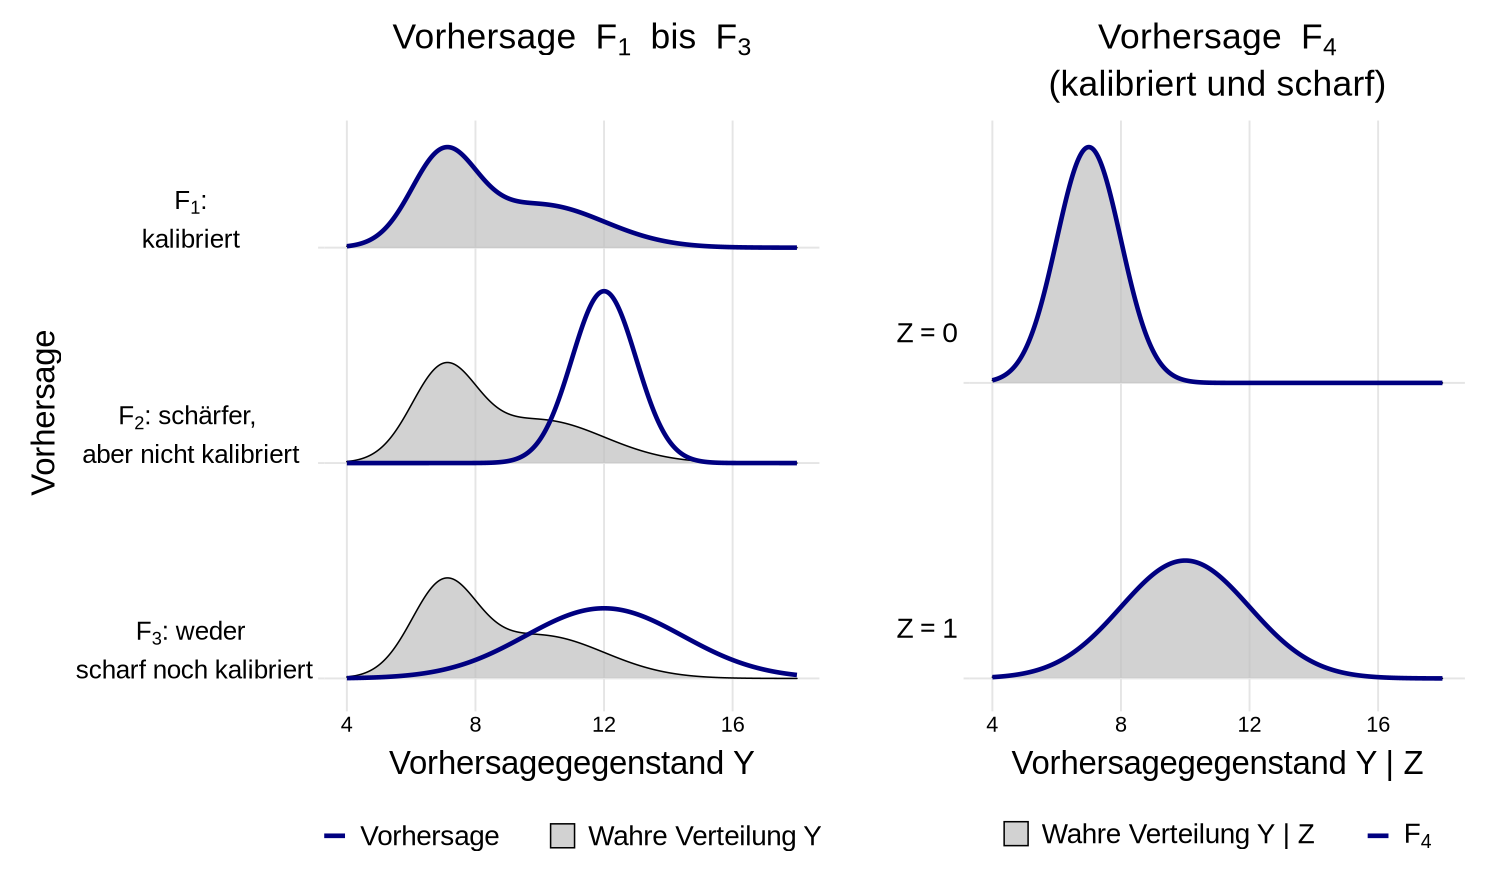
\includegraphics[width=\linewidth]{figs/cal_sharp_visu_Rplot.png}
    \caption{ Verteilung der Vorhersagen im Vergleich zur wahren Verteilung aus Beispiel \ref{bsp:cal_sharp}.
    }
    \label{fig:cal_sharp_visu}
\end{figure}{}

Zur quantitativen Gesamtbewertung der Vorhersagegüte werden schließlich Scoring-Rules oder Scores verwendet \parencite{gneitingMakingPoint2011}. Dabei handelt es sich um Funktionen, die einer probabilistischen Vorhersage anhand von Verifikationsdaten einen numerischen Wert zuordnen. Auf diese Weise lassen sich unterschiedliche Vorhersagen einfach vergleichen; ein besserer Score entspricht einer höheren Vorhersagegüte. Zudem lassen sich einige Scores in Komponenten zerlegen, die wiederum Kalibrierung und Schärfe getrennt widerspiegeln, wodurch Stärken und Schwächen von Vorhersagen deutlich werden können \parencite{arnold2024decompositions}.




\chapter{Klassische Kalibrierungskonzepte}\label{chap:classic_calibration}
In diesem Kapitel widmen wir uns dem ersten wichtigen Kriterium zur Evaluation probabilistischer Vorhersagen: der Kalibrierung. Hierzu führen wir drei grundlegenden Begriffe der Kalibrierung ein. Die formale Definition des Vorhersageraums aus Definition \ref{def::room} dient dabei als Rahmen, innerhalb dessen wir diese Begriffe definieren. Im Mittelpunkt steht insbesondere die Frage, wie sich die stochastische Konzeption von Kalibrierung empirisch übersetzten lässt. Schließlich werden dazu Reliabilitätsdiagramme vorgestellt, die eine visuelle, empirische Beurteilung der Kalibrierung ermöglichen.

\section{Auto-Kalibrierung} \label{sec:auto_cal}
Im Folgenden beschreiben wir mit $\mathcal{L}$ eine bedingte oder unbedingte Wahrscheinlichkeitsverteilung identifiziert durch ihre Verteilungsfunktion. Wir schreiben \[\mathcal{L}(Y \mid F)\coloneqq\mathcal{L}(Y \mid \sigma(F))\] für die bedingte Verteilung von $Y$ gegeben der, durch die Vorhersage $F$ erzeugten $\sigma$-Algebra.

\begin{defi}[Auto-Kalibrierung \parencite{gneiting2023regression}]
\label{def::auto}
Eine Vorhersage $F$ heißt \emph{auto-kalibriert} bzgl. $Y$, wenn sie, gegeben der von ihr verwendeten Information, ideal ist. D.h.
\begin{equation}
\LW(Y \mid F) = F \qquad \text{fast sicher}
\end{equation}
oder äquivalent
\begin{equation}\label{eq:auto}
\forall y \in \R: \;  \PW(Y \le y \mid F) = F(y) \qquad \text{fast sicher}.
\end{equation}{}
\end{defi}

Eine auto-kalibrierte Vorhersage reproduziert somit exakt die Struktur des Vorhersagegegenstands, gegeben der Information, die die Vorhersage nutzt; sie nutzt ihre Information optimal. Bei der Überprüfung von Vorhersagen hinsichtlich ihrer Kalibrierung ist Auto-Kalibrierung daher das eigentliche Ziel.

\begin{bsp}[Ideale und marginale Vorhersage sind auto-kalibriert \texorpdfstring{\parencite[Example 2.4]{gneitingCombining2013,Gneiting2007}})]  \label{bsp:auto_kal}
Sei $Y$ ein Vorhersagegegenstand mit 
\[
Y = \mu + \varepsilon \quad \text{wobei} \quad \mu,\; \varepsilon \sim \N(0,1), \quad \mu \indep \varepsilon.
\]
Dabei kann $\mu$ als zufälliger latenter Zustand (z.B. letzter Zustand der Atmosphäre) und $\varepsilon$ als unabhängiges Rauschen interpretiert werden. Wir betrachten jetzt zwei probabilistische Vorhersagen.
\begin{itemize}
    \item Sei $F_1 \coloneqq \N(\mu,1)$. Wir nennen $F_1$ die \emph{ideale Vorhersage}, weil sie den Zustand $\mu$ kennt und optimal verwendet. Daraus ergibt sich die zugehörige Information $\sigma(F_1)=\sigma(\mu)$.
    \item Sei $F_2 \coloneqq \N(0,2)$ die zweite Vorhersage. Wir bezeichnen sie als \emph{marginale Vorhersage}. Sie ist konstant und verwendet keine zusätzliche Information. Daher ist die zugehörige Informationsmenge die triviale $\sigma$-Algebra,  $\sigma(F_2)=\{\emptyset, \Omega\}$.
    \item Für die bedingten Vorhersagen erhalten wir
        \begin{align*}
            \LW(Y \mid F_1)&=\LW(Y \mid \mu)=\N(\mu,1), \\
            \LW(Y \mid F_2)&=\LW(Y)=\N(0,2).
        \end{align*}
    Somit sind sowohl $F_1$ als auch $F_2$ jeweils auto-kalibriert.
\end{itemize}
Dieses Beispiel verdeutlicht außerdem, dass Auto-Kalibrierung allein nicht ausreicht, um die Qualität einer Vorhersage zu bewerten. Obwohl sowohl $F_1$ als auch $F_2$ auto-kalibriert sind, liefert $F_1$ aufgrund der zusätzlichen Information über $\mu$ die deutlich präzisere (schärfere) und damit bessere Vorhersage. 
\end{bsp}{}


Für kontinuierliche Größen wie Temperatur gibt es im Allgemeinen empirisch keine gute Möglichkeit, Auto-Kalibrierung direkt zu überprüfen \parencite{gneitingCombining2013}, weshalb Auto-Kalibrierung eher ein theoretisches Ideal ist. Der Grund hierfür ist, dass sich die Vorhersageverteilungen in der Praxis häufig von Beobachtung zu Beobachtung unterscheiden, sodass die bedingte Verteilung von $Y$ gegeben $F$ empirisch nicht zuverlässig, selbst mit vielen Daten, geschätzt werden kann. Daher greift man auf andere, schwächere Konzepte der Kalibrierung zurück. Im Folgenden führen wir hierzu die probabilistische und die marginale Kalibrierung ein.

%independence erläutern
%Vielleicht noch isotone Kalibrierung erwähen


\section{Marginale Kalibrierung}\label{sec:marg_cal}
\subsection{Definition}
Eine erste einfache Möglichkeit zur Überprüfung von Kalibrierung besteht darin zu untersuchen, ob Vorhersagegegenstand und Vorhersage im Mittel (d.h. über alle Vorhersagesituationen hinweg) dieselbe Verteilung besitzen. Diese Form der Kalibrierung bezeichnen wir als \emph{marginale Kalibrierung}.

\begin{defi}[Marginale Kalibrierung \parencite{gneiting2023regression}]
Die Vorhersage $F$ heißt \emph{marginal kalibriert}  bzgl. $Y$, falls
\[
\forall y \in \R: \; \; \PW(Y \leq y) = \E_\PW \big[F(y)\big],
\]
wobei der Erwartungswert bezüglich der zufälligen Vorhersage $F$ gebildet wird.
\end{defi}{}

%Marginale Kalibrierung bedeutet, dass die marginale Verteilung der Vorhersagen mit der marginalen Verteilung des Vorhersagegegenstands übereinstimmt.


\subsection{Empirische Überprüfung}
Empirisch betrachten wir nun Vorhersage-Beobachtungspaare der Form \eqref{eq:stich}. Zunächst definieren wir empirische Versionen der marginalen Vorhersageverteilung und der marginalen Verteilungsfunktion des Vorhersagegegenstands.

%gneiting resin 2023
\begin{defi}[Empirisch marginale Vorhersageverteilung und empirisch marginale Verteilung des Vorhersagegegenstandes \parencite{gneiting2023regression}]
Seien Vorhersage-Beobachtungspaare der Form \eqref{eq:stich} gegeben und $y \in \R$. Dann lautet die empirische marginale Vorhersage oder mittlere Vorhersage
\begin{equation} \label{eq:F_mg}
   \hat{F}_{mg}(y)\coloneqq\frac{1}{n}\sum_{i=1}^{n}F_i(y). 
\end{equation}
Die empirisch marginale Verteilung des Vorhersagegegenstandes schreiben wir als
\begin{equation} \label{eq:Y_mg}
\widehat{\PW}(Y \leq y)\coloneqq\frac{1}{n}\sum_{i=1}^{n}\mathds{1}\{y_i\leq y\}.
\end{equation}

\end{defi}

Für Temperaturvorhersagen bedeutet dies, dass die über die betrachteten Vorhersagezeitpunkte oder Orte aggregierte Verteilung der vorhergesagten Temperaturen mit der entsprechenden marginalen Verteilung der tatsächlich beobachteten Temperaturen übereinstimmt. Die Vorhersage erfasst damit das zugrunde liegende Klimaniveau \parencite{Gneiting2007}.

Marginale Kalibrierung können wir jetzt visuell überprüfen, indem wir die mittlere Vorhersage gegen die empirische marginale Verteilungsfunktion des Vorhersagegegenstands abbilden. Wir nennen diese Darstellung das \emph{marginale Reliabilitätsdiagramm} \parencite[B.3]{gneiting2023regression}. Liegen die Werte annähernd auf der Diagonalen, ist die marginale Kalibrierung erfüllt. Eine $S$-förmige Abweichung deutet auf eine überdispersive, während eine inverse $S$-Form auf eine unterdispersive marginale Vorhersage hinweist. Zusätzlich weist eine systematische Verschiebung der Kurve über oder unter der Diagonalen auf einen Bias in der Vorhersage hin. Das folgende Beispiel illustriert die Interpretation des Diagramms für  nicht marginal kalibrierte Vorhersagen.

% überdispersive Vorhersage mit negativem Bias, $F = \N(3,50)$; überdispersive Vorhersage mit positivem Bias, $F = \N(7,50)$.

\begin{bsp}[Interpretation des marginalen Reliabilitätsdiagramms] \label{bsp:marg_cal}
Zur Veranschaulichung der Interpretation marginaler Reliabilitätsdiagramme betrachten wir eine Zufallsvariable
\[
Y \sim \N(5,25).
\]
Abbildung \ref{fig:marg_cal} zeigt die marginalen Reliabilitätsdiagramme acht verschiedener statischer probabilistischer Vorhersagen mit prototypischen Fehlern. Hierzu wurden $500$ unabhängige Beobachtungen von $Y$ simuliert und mit den statischen Vorhersagen zu Vorhersage-Beobachtungspaaren zusammengeführt. Dadurch lassen sich verschiedene Formen der Abweichungen von marginalen Kalibrierung veranschaulichen. Wir betrachten folgende Vorhersagen:
\begin{itemize}
\item[(a)] eine unterdispersive Vorhersage $F=\N(5,8)$, bei der die vorhergesagte Varianz kleiner als die tatsächliche Varianz von $Y$ ist.

\item[(b)] eine überdispersive Vorhersage $F=\N(5,50)$, bei der die vorhergesagte Varianz größer als die tatsächliche Varianz ist.

\item[(c)] mit $F=\N(3,25)$ liegt der Erwartungswert der Vorhersage unterhalb des tatsächlichen Erwartungswerts. Es liegt daher ein negativer Bias vor.

\item[(d)] mit $F=\N(7,25)$ liegt der Erwartungswert der Vorhersage oberhalb des tatsächlichen Erwartungswerts, sodass ein positiver Bias vorliegt.

\item[(e)] und (f) kombinieren die zu geringe Streuung aus (a) mit dem negativen bzw. positiven Bias aus (c) bzw. (d).

\item[(g)] und (h) kombinieren die zu hohe Streuung aus (b) mit einem negativen bzw. positiven Bias aus (c) bzw. (d).
\end{itemize}
Wie Abbildung \ref{fig:marg_cal} zu entnehmen ist, lassen sich zusätzlich approximativ Konsistenzbänder einzeichnen. Die Bänder dienen dazu, zu beurteilen, ob die beobachteten Abweichungen von der marginalen Kalibrierung noch mit zufallsbedingten Schwankungen vereinbar sind. Diese wurden hier nach der Methode von \textcite{gneiting2023regression} unter Annahme marginaler Kalibrierung über ein Resampling-Verfahren auf Basis von $1000$ Replikationen erstellt. Das Verfahren ist in Appendix \ref{seq:consist_marg} beschrieben.
\end{bsp}

\begin{figure}
    \centering
    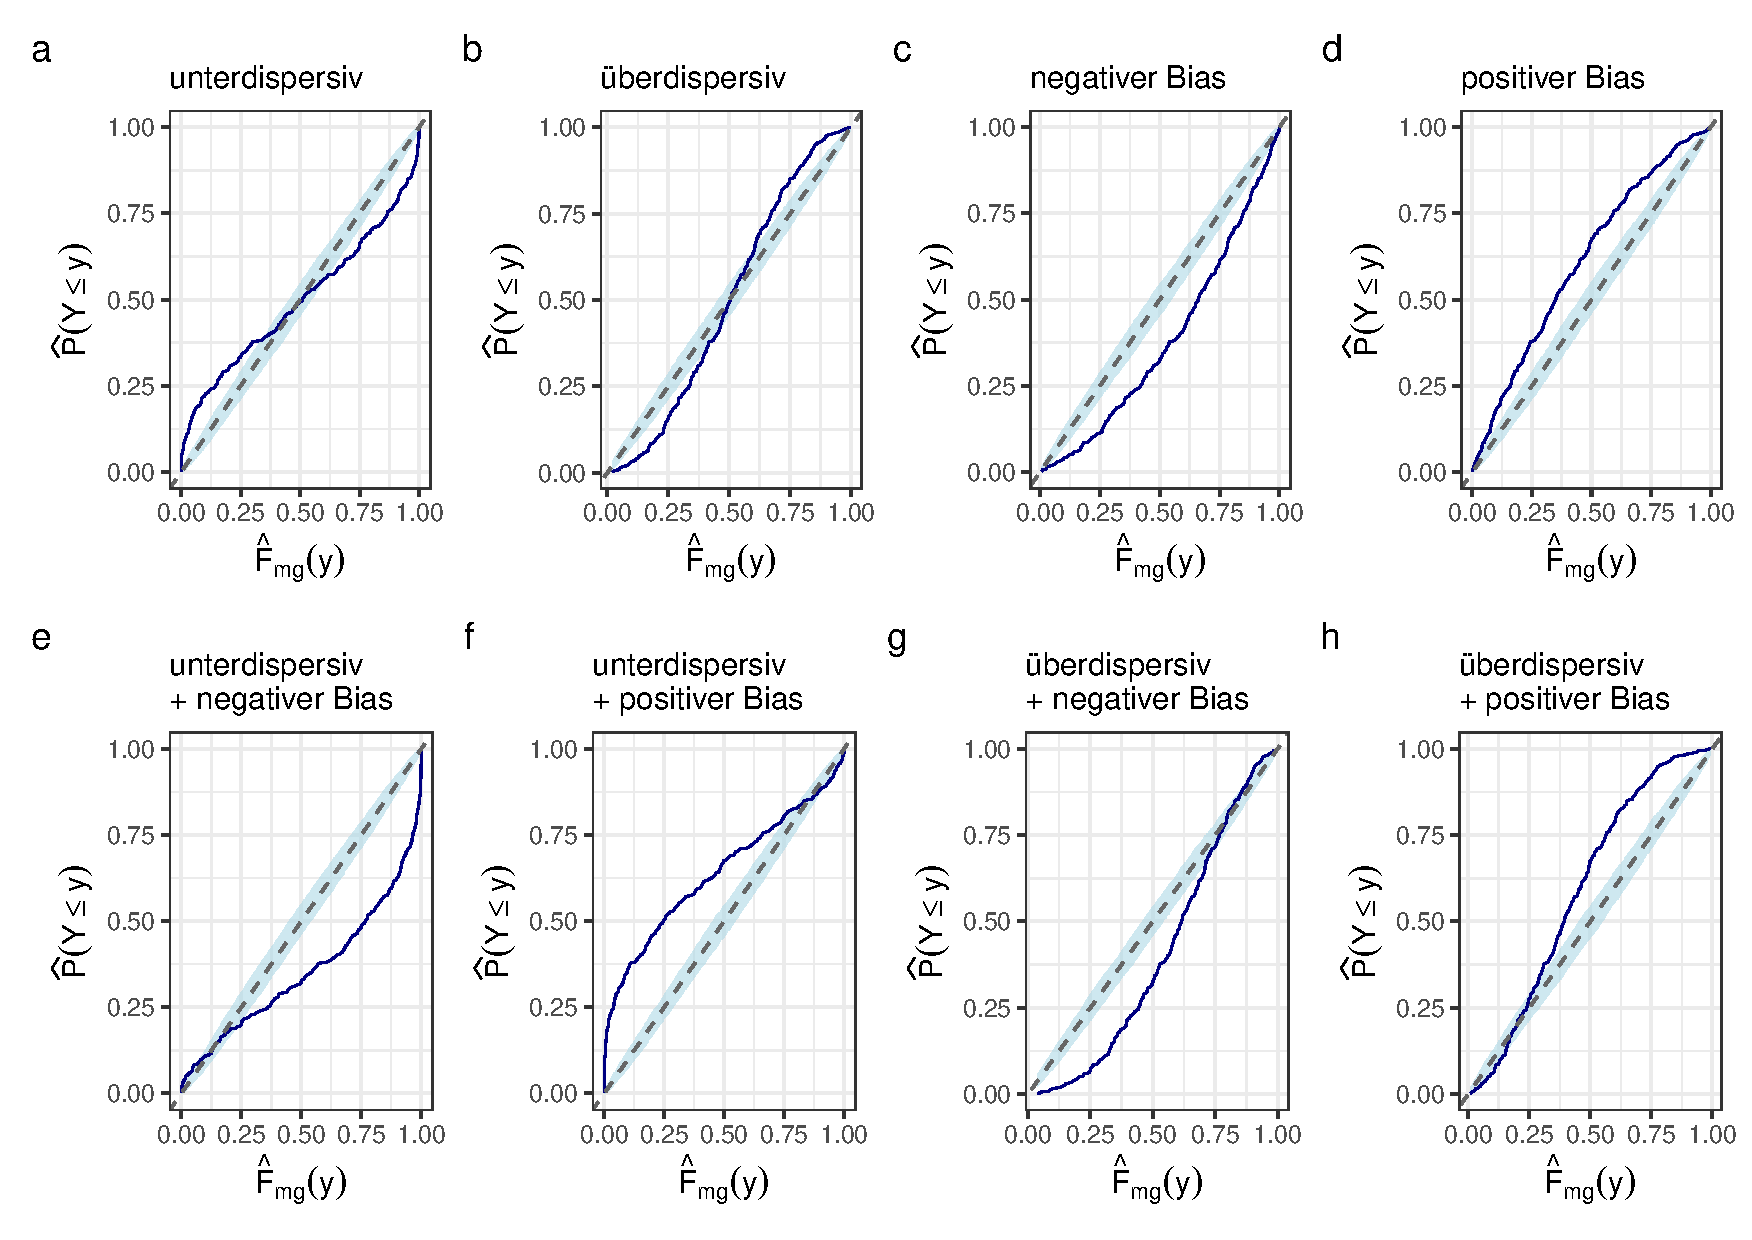
\includegraphics[width=\linewidth]{figs/marg_theo_Rplot.pdf}
    \caption{
    Marginale Reliabilitätsdiagramme zum Beispiel \ref{bsp:marg_cal}.
    }
    \label{fig:marg_cal}
\end{figure}{}


\FloatBarrier
\section{Probabilistische Kalibrierung} \label{sec:pit_cal}
\subsection{Definition} \label{sec:def_prob}
Zur Motivation probabilistischer Kalibrierung betrachten wir zunächst eine grundlegende Eigenschaft von Verteilungsfunktionen. Sei
$X \sim G$
eine Zufallsvariable mit stetiger Verteilungsfunktion $G$. 
Setzten wir nun die Zufallsvariable $X$ selbst in ihre Verteilungsfunktion $G$ ein, erhalten wir die transformierte Zufallsvariable
\begin{equation} \label{eq:pit_intro}
    G(X)
\end{equation}
Für eine stetige Verteilungsfunktion ist diese transformierte Zufallsvariable uniform gleichverteilt \parencite[Theorem 2.1.10]{CasellaBerger2002}. Sie wird als \emph{Wahrscheinlichkeitsintegraltransformation} (engl. \emph{probability integral transform}, PIT) bezeichnet \parencite{gneitingCombining2013}.

Wir können diese Eigenschaft nun nutzen, um die Güte einer probabilistischen Vorhersage zu beurteilen. Dafür betrachten wir wieder einen  Vorhersageraum $(F,Y)$. Ist die Vorhersage $F$ tatsächlich eine passende Beschreibung der Verteilung von $Y$, sollte sich $Y$ unter Anwendung der PIT genauso verhalten wie eine Beobachtung aus $F$. Daher Fordern wir: Eine Vorhersage $F$ ist probabilistisch kalibriert, sofern diese PIT-transformierte Zufallsvariable standarduniformverteilt ist. Also
\[
F(Y) \sim \mathcal{U}(0,1).
\]
Zwei Aspekte sind hier zusätzlich zu berücksichtigen. Besitzt die Verteilungsfunktion, in die die Zufallsvariable im Rahmen der PIT eingesetzt wird, Sprungstellen,  gilt die Gleichverteilung der PIT im Allgemeinen nicht, selbst wenn die Zufallsvariable tatsächlich dieser Verteilung folgt. Wir verallgemeinern daher die PIT auf beliebige Zufallsvariablen, indem wir eine randomisierte Version der Transformation betrachten \parencite{ferguson1967}. Hierzu erweitern wir den Vorhersageraum aus Definition \ref{def::room} um eine von $F$ und $Y$ unabhängige Zufallsvariable $U\sim\mathcal{U}(0,1)$ und betrachten Tupel der Form
\[
(F,Y,U).
\]
Der zweite Aspekt ist, dass im Vorhersageraumsetting die Vorhersage $F$ im Gegensatz zu $G$ in \eqref{eq:pit_intro} nicht fixiert, sondern selbst eine Zufallsgröße ist. Damit können wir nun die randomisierte PIT im Vorhersageraum definieren.


\begin{defi}[Wahrscheinlichkeitsintegral\-transfor\-ma\-tion, PIT \parencite{gneiting2023regression}]
Die Zufallsvariable $Z_F$ nennen wir Wahrscheinlichkeitsintegraltransformation (PIT) falls
\begin{equation}\label{eq:PIT}
Z_F=F(Y^-)+U(F(Y)-F(Y^-)),
\end{equation}{}wobei $F(y^-) := \lim_{x \rightarrow y^-} F(x)$ den linksseitigen Grenzwert von $F$ bezeichnet. Ist $F$ stetig, so vereinfacht sich das zu
\[
Z_F = F(Y).
\]
\end{defi}{}

\begin{defi}[Probabilistische Kalibrierung \parencite{gneiting2023regression}]
Die Vorhersage $F$ heißt \emph{probabilistisch kalibriert} bzgl. $Y$, falls
\begin{equation}\label{eq:PK1}
    Z_F \sim \mathcal{U}(0, 1) 
\end{equation}{}
oder äquivalent
\begin{equation}\label{eq:PK2}
\forall \alpha \in (0,1): \PW\big(Z_F \leq \alpha \big) = \alpha
\end{equation}{}
gilt.
\end{defi}{}

\subsection{Empirische Überprüfung}
Empirisch betrachten wir nun wieder Beobachtungen der Form \eqref{eq:stich}. Zunächst definieren wir empirische Versionen der PIT-Zufallsvariable und ihre Verteilungsfunktion.

\begin{defi}[Empirisches PIT und empirische PIT Verteilung] Seien $u_1,\dotsc,u_n$ unabhängige Realisierungen von $U$.
Die empirischen PIT-Werte erhalten wir, indem wir \eqref{eq:PIT} auf Ebene der Tupel $(F_i,y_i,u_i)$ anwenden. Es gilt
    \[
        z_i \coloneqq F_i(y_i^-) + u_i \cdot \bigl(F_i(y_i) - F_i(y_i^-)\bigr), \quad i = 1,\dots,n.
    \]
    Sind alle $F_i$ stetig, verwenden wir stattdessen
    \[
        z_i \coloneqq F_i(y_i).
    \]
    Die empirische PIT Verteilung lautet dann für $\alpha \in (0,1)$
    \begin{equation} \label{eq:emp_pit_dist}
        \widehat{\PW}(Z_F \leq \alpha) = \frac{1}{n}\sum_{i=1}^{n}\mathds{1}\{z_i\leq \alpha\}.
    \end{equation}
\end{defi}{}

Visuell können wir probabilistische Kalibrierung auf zwei verschiedene Arten überprüfen. Die erste (klassische und verbreitete) Variante ist das \emph{PIT-Histogramm} \parencite{gneiting2014probabilistic,gneitingCombining2013}. Hier überprüfen wir probabilistische Kalibrierung in der Darstellung gemäß \eqref{eq:PK1}, indem wir die empirischen PIT Werte in Form eines auf Dichte normierten Histogramms darstellen. Probabilistische Kalibrierung ist erfüllt, sofern das PIT-Histogramm annähernd flach ist. U-förmige Histogramme weisen auf unterdisperse Vorhersageverteilungen hin, während glockenförmige Histogramme auf überdisperse Vorhersageverteilungen deuten.

Die zweite Variante entspricht der Überprüfung von \eqref{eq:PK2}. Hierbei stellen wir die empirische PIT Verteilungsfunktion  \eqref{eq:emp_pit_dist} graphisch dar. Wir nennen diese Variante das \emph{PIT-Reliabilitätsdiagramm}. Der Vorteil gegenüber dem PIT-Histogramm besteht darin, dass die Darstellung nicht von der Wahl der Bins abhängt, weil unterschiedliche Binnings zu variierenden visuellen Eindrücken führen und dadurch Kalibrierungsfehler entweder verdecken oder scheinbar verstärken können \parencite{gneiting2023regression}. Das PIT-Reliabilitätsdiagramm interpretieren wir analog zum marginalen Reliabilitätsdiagramm. Abbildung \ref{fig:pit_cal} illustriert schematische Beispiele zur Einordnung des Reliabilitätsdiagramms und Histogramms.


\begin{bsp}[Interpretation des PIT-Reliabilitätsdiagramms und des PIT-Histogramms] \label{bsp:pit_cal}
Zur Veranschaulichung der Interpretation von PIT-Reliabilitäts\-diagramm und PIT-Histo\-gramm betrachten wir den Vorhersage\-gegenstand und die Vorhersagen aus Beispiel \ref{bsp:marg_cal}. In Abbildung \ref{fig:pit_cal} sind die zu den Vorhersagen korrespondierenden PIT-Reliabilitätsdiagramme und PIT-Histogramme dargestellt. Die PIT-Histogramme wurden jeweils mit $20$ Bins erstellt. Die folgenden Vorhersagen sind den jeweiligen Plots zugeordnet:
%checken, das das wirklich richtig zugeordnet ist
\begin{itemize}
\item[(a-b)] die unterdispersive Vorhersage.

\item[(c-d)] die überdispersive Vorhersage.

\item[(e-f)] die Vorhersage mit negativem Bias.

\item[(g-h)] die Vorhersage mit positivem Bias.

\item[(i-j)] und (m-n) unterdispersive Vorhersagen mit negativem beziehungsweise positivem Bias.

\item[(k-l)] und (o-p) uberdispersive Vorhersagen mit negativem beziehungsweise positivem Bias.

\end{itemize}
Dem Reliabilitätsdiagramm können wir wieder ein Konsistenzband anfügen. Das hier verwendete Verfahren ist in Appendix \ref{seq:consist_pit} beschrieben.
\end{bsp}

\begin{figure}
    \centering
    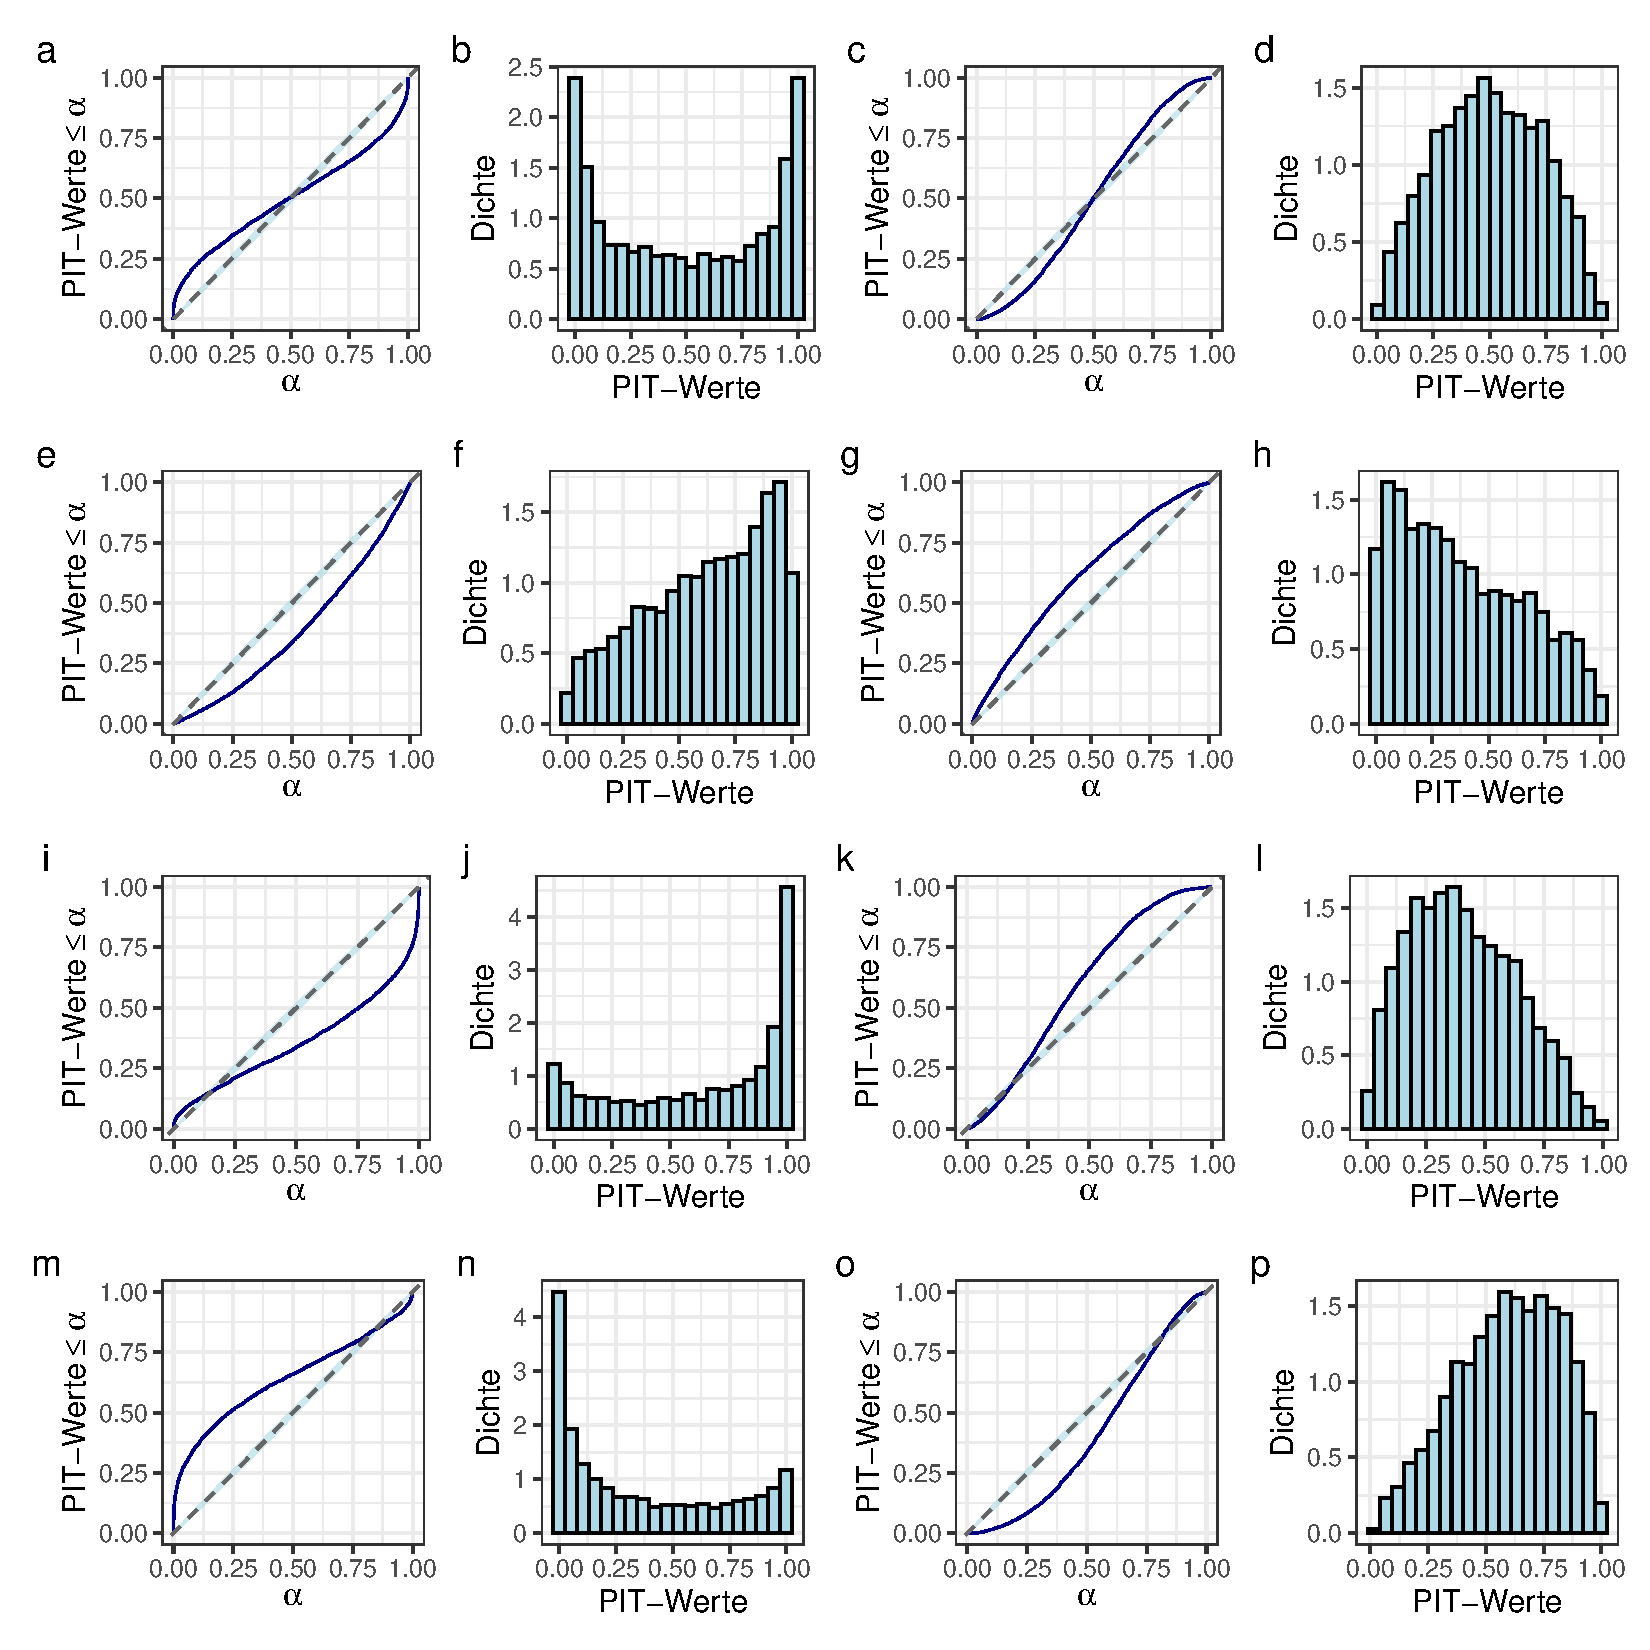
\includegraphics[width=\linewidth]{figs/pit_Rplot.pdf}
    \caption{
    Abbildung zum Beispiel \ref{bsp:pit_cal} zur Interpretation des PIT-Reliabi\-litätsdiagramms und PIT-Histogramms.
    }
    \label{fig:pit_cal}
\end{figure}{}


Der im Reliabitlitäsdiagramm gemachte Vergleich von $\widehat{\PW}(Z_F \leq \alpha)$ mit $\alpha$ ermöglicht zudem eine anschauliche Interpretation über die verschiedenen Vorhersagesituationen hinweg. Liegt beispielsweise für $\alpha=0.75$ die empirische PIT Verteilung bei \mbox{$\widehat{\PW}(Z_F\leq 0.75)=0.9$}, so liegen etwa 90\% der beobachteten Realisierungen unterhalb des jeweils vorhergesagten 75\%-Quantilniveaus. Dies deutet darauf hin, dass das 75\%-Quantil über die betrachtete Stichprobe hinweg überschätzt wird. Liegt die empirische PIT Verteilung dagegen bei $0.6$, deutet dies entsprechend auf ein unterschätztes 75\%-Quantil hin. Für das Diagramm bedeutet dies, dass Werte oberhalb der Diagonalen darauf hindeuten, dass die entsprechenden Quantile über die betrachtete Stichprobe hinweg überschätzt werden, Werte unterhalb der Diagonalen deuten tendenziell auf unterschätzte Quantile. Damit lässt sich bereits erkennen, dass die probabilistische Kalibrierung eng mit der (unbedingten) Quantilkalibrierung zusammenhängt, auf die wir im Folgenden Kapitel genauer eingehen.


\chapter{Quantilkalibrierung} \label{chap:quant_cal}
Im vorherigen Kapitel haben wir uns mit klassischen Kalibrierungsbegriffen befasst. Eine alternative Perspektive ergibt sich, wenn wir Kalibrierung auf Basis statistischer Funktionale betrachten, insbesondere zur Untersuchung bedingter Kalibrierung. Stellvertretend betrachten wir hierfür die Quantilkalibrierung, die im Folgenden detailliert vorgestellt wird.

In Abschnitt \ref{seq:T_cal} stellen wir die Grundidee der Kalibrierung auf statistischen Funktionalen vor. Anschließend betrachten wir Quantilkalibrieung in Abschnitt \ref{seq:Quantcal}. Dort führen wir zunächst den Begriff der unbedingten und bedingten $\alpha$-Quantilkalibrierung ein, bevor wir uns mit der empirischen Überprüfung von Quantilkalilbrierung in beschäftigen. Für die Untersuchung der bedingten Quantilkalibrierung erläutern wir dabei den CORP-Ansatz von \textcite{gneiting2023regression}.

\section{Kalibrierung auf statistischen Funktionalen} \label{seq:T_cal}
Bei den bisher eingeführten Kalibrierungsbegriffen haben wir jeweils die gesamte Verteilung des Vorhersagegegenstands sowie der Vorhersage betrachtet. Stattdessen kann Kalibrierung auch anhand einzelner Charakteristika einer probabilistischen Vorhersage untersucht werden, etwa des Erwartungswerts, auf Grundlage von Schwellenwerten oder Quantilen \parencite{gneiting2023regression, jordanOptimalSolutions2022}.

Das hat mehrere Vorteile. Erstens sind solche Betrachtungen oft einfacher und leichter zu interpretieren. Beispielsweise bedeutet die Kalibrierung des Erwartungswertes, dass der Erwartungswert der Vorhersage und Erwartungswert des Vorhersagegegenstands übereinstimmen. Zweitens liegt das Interesse in vielen Anwendungen nicht auf der voll\-ständigen Vorhersageverteilung, sondern nur auf bestimmten Aspekten der Verteilungen, etwa darauf, ob das 25\%- oder 75\%-Quantil korrekt getroffen wird. Drittens ermöglicht dieser Zugang eine natürliche Formulierung bedingter Kalibrierung. Anstatt wie bei der Auto-Kalibrierung auf die gesamte Vorhersage zu konditionieren, wird lediglich auf das vorhergesagte statistische Funktional bedingt. Im Fall des Erwartungswerts bedeutete es, dass der Erwartungswert des Vorhersagegegenstands bedingt auf den vorhergesagten Erwartungswert diesem entspricht. Anschaulich entspricht das der Situation, dass alle Tage mit einer vorhergesagten Durchschnittstemperatur von $20\C$ im Mittel auch tatsächlich eine Temperatur von $20\C$ aufweisen.

Gerade der letzte Aspekt ist für die Überprüfung von Kalibrierung bedeutend, denn marginale und probabilistische Kalibrierung sind unbedingt. Eine ausschließlich auf solchen unbedingten Kalibrierungsbegriffen basierende Evaluation gilt jedoch zunehmend als unzureichend  \parencite{gneiting2023regression}.

Wenn wir nur einzelne Funktionale betrachten, entspricht das der Überprüfung von Punktvorhersagen. Das erlaubt noch keine umfassende Aussage über die gesamte probabilistische Vorhersage. Deshalb betrachten wir einzelne Funktionale nicht allein, sondern Klassen ähnlicher Funktionale, etwa eine Menge an Quantilen bzw. Schwellenwerten, gemeinsam. Dadurch lassen sich Rückschlüsse über ganze Vorhersageverteilungen ziehen.

Im Rahmen der vorliegenden Arbeit konzentrieren wir uns auf die Quantilkalibrierung. Gegenüber der Schwellenwertkalibrierung besitzt sie den Vorteil, unabhängig von der Einheit des Vorhersagegegenstands zu sein \parencite{bentzienDecomposition2014}. Allerdings sind Quantile im Allgemeinen nicht notwendig reellwertig, sondern können mengenwertig auftreten.  Im Folgenden wollen wir jedoch mit reellen Werten arbeiten. Dazu müssen wir die Definition von Quantilkalibrierung entsprechend einschränken.


\section{Quantilkalibrierung} \label{seq:Quantcal}
\subsection{Definiton}
Quantile können mengenwertig sein. Das kann genau dann eintreten, wenn die Verteilungsfunktion nicht streng monoton wächst, sondern auf einem Intervall flach ist oder Sprünge besitzt. Daher unterscheiden wir zwischen unterem und oberem $\alpha$-Quantil \parencite{gneiting2023model}.

\begin{defi}[Unteres und oberes $\alpha$-Quantil  \parencite{gneiting2023model}]
Sei $\alpha \in (0,1)$. Für eine Verteilungsfunktion $F$ definieren wir das untere $\alpha$-Quantil als
\begin{equation}\label{eq:lowerquantile}
    q^-_\alpha(F)
    \coloneqq
    \sup \{ x \in \R : F(x) < \alpha \}
    =
    \inf \{ x \in \R : F(x) \ge \alpha \},
    \end{equation}
    sowie das obere $\alpha$-Quantil als
    \begin{equation}\label{eq:upperquantile}
    q^+_\alpha(F)
    \coloneqq
    \inf \{ x \in \R : F(x) > \alpha \}.
\end{equation}
\noindent
\begin{itemize}
    \item Für das untere Quantil $q^-_\alpha(Y)$ schreiben wir im Folgenden einfach nur  $q_\alpha(Y)$.
    \item Ein gültiges $\alpha$-Quantil von $F$ ist dann ein beliebiges Element aus der Menge 
    \[
    \left[q_\alpha(F),q^+_\alpha(F)\right]
    \].
\end{itemize}
\end{defi}
\noindent
Analog schreiben wir für den Vorhersagegegenstand $Y$ \begin{align*}
    q_\alpha(Y) &\coloneqq  q_\alpha(\LW(Y)) = \inf \{ x \in \R : \PW(Y \le x) \ge \alpha \},\\
    q^+_\alpha(Y)&\coloneqq q^+_\alpha(\LW(Y)) = \inf \{ x \in \R : \PW(Y \le x) > \alpha \}.
\end{align*}
Schließlich bezeichnen wir mit $\hat q_\alpha(\cdot)$ den empirischen Schätzer des unteren $\alpha$-Quantils $q_\alpha(\cdot)$. Zu dessen Berechnung verwenden wir in der vorliegenden Arbeit Definition 1 aus \textcite{hyndman1996sample}, nach der das empirische $\alpha$-Quantil durch die verallgemeinerte Inverse der empirischen Verteilungsfunktion gegeben ist.
 
Als nächstes führen wir die Quantilkalibrierung ein. In der Literatur finden sich jedoch leicht verschiedene, eng verwandte Definitionen dieser, die wir im Folgenden auflisten. Wir unterscheiden zwischen einer unbedingten Variante, die keine weitere Vorhersageinformation nutzt und einer bedingten. 

\begin{defi}[$\alpha$-Quantilkalibrierung]
Eine Vorhersage $F$ heißt \emph{unbedingt $\alpha$-quantil\-kalibriert} für ein $\alpha  \in (0,1)$  bzgl. $Y$   falls
\begin{equation}\label{eq:uncond_pm_quant_cal}
    \PW(Y \leq q_\alpha(F)) \ge \alpha \quad \text{und} \quad  \PW(Y < q^+_\alpha(F)) \leq \alpha
\end{equation}
gilt. Diese Darstellung entspricht Gleichung (10) aus \textcite{gneiting2023regression}. 

Die \emph{unbedingte $\alpha$-Quantilkalibrierung} überprüft also, ob die vorhergesagten $\alpha$-Quantile $q^\pm_{\alpha}(F)$ die korrekten marginalen Überdeckungswahrscheinlichkeiten aufweisen. Im Rahmen des Vorhersageraums ist die Vorhersage $F$ als Markovkern zufallsabhängig. Daher sind auch die induzierten Quantile $q^\pm_{\alpha}(F)$ im Allgemeinen wieder Zufallsvariablen. Die unbedingte $\alpha$-Quantilkalibrierung ist daher eine marginale Eigenschaft der gemeinsamen Verteilung $(F,Y)$. Wir betrachten nun eine leicht abgeschwächte Variante, die ausschließlich auf dem unteren vorhergesagten Quantil basiert:
\begin{equation}\label{eq:unb_quantcal_lower}
    \quad \PW(Y \leq q_\alpha(F)) \ge \alpha \quad \text{und} \quad  \PW(Y < q_\alpha(F)) \leq \alpha.
\end{equation}{}
Diese Einschränkung stellt in der Praxis keine wesentliche Einbuße dar, weil die Quantile in den meisten Fällen eindeutig sind \parencite{arnold2025isotonic}. Sie hat jedoch den Vorteil, dass wir immer eindeutige Werte für die vorhergesagten $\alpha$-Quantile verwenden.

Für \emph{bedingte $\alpha$-Quantilkalibrierung}, bedingen wir \eqref{eq:unb_quantcal_lower} auf das vorhergesagte $\alpha$-Quantil. Die Vorhersage $F$ heißt bedingt $\alpha$-quantilkalibriert für ein $\alpha \in (0,1)$ bzgl. $Y$ falls
\begin{equation}\label{eq:cond_quantcal_lower}
    \quad \PW(Y \leq q_\alpha(F) \mid q_\alpha(F)) \ge \alpha \quad \text{und} \quad  \PW(Y < q_\alpha(F) \mid q_\alpha(F)) \leq \alpha
\end{equation}{}
gilt.
Diese Definition entspricht Gleichung (2) aus \textcite{gneiting2023model}.
Im Gegensatz zur unbedingten Quantilkalibrierung wird hier nicht nur die marginale Überdeckungs\-wahrscheinlichkeit betrachtet. Stattdessen prüfen wir, ob die Vorhersagen auch bedingt auf das jeweils vorhergesagte Quantil korrekt kalibriert sind.

Die Bedingung in \eqref{eq:cond_quantcal_lower} kontrolliert weiterhin Überdeckungswahrscheinlichkeiten. Eine leicht stärkere Forderung besteht darin zu verlangen, dass das vorhergesagte Quantil exakt dem entsprechenden Quantil der bedingten Verteilung von $Y$ entspricht. Dies führt zur folgenden Definition gemäß Gleichung (10) aus \textcite{arnold2025isotonic}. Sie lautet: Die Vorhersage $F$ heißt \emph{bedingt $\alpha$-quantilkalibriert} für ein $\alpha \in (0,1)$ bzgl. $Y$ falls
\begin{equation}\label{eq:cond_alpha_quant_cal}
\quad q_\alpha\left(Y \mid q_\alpha(F)\right) = q_\alpha(F)\quad \text{fast sicher}
\end{equation}
gilt. Es besteht Äquivalenz zu \eqref{eq:cond_quantcal_lower}, sofern das bedingte $\alpha$-Quantil von $Y$ eindeutig ist. 

Diese letzte Darstellung führen wir ein, weil sie in direkter Nähe zur empirischen Überprüfung der bedingten $\alpha$-Quantilkalibrierung steht, die wir mithilfe eines Reliabilitätsdiagramms umsetzen werden. Zudem bietet sie eine unmittelbare intuitive Interpretation: Immer wenn ein $\alpha$-Quantil von beispielsweise $10\C$ vorhergesagt wird, soll auch das tatsächliche $\alpha$-Quantil der bedingten Verteilung bei $10\C$ liegen.
\end{defi}{}

Aktuell betrachten wir nur ein einziges $\alpha$-Quantil. Das entspricht der Überprüfung einer Punktvorhersage und lässt somit noch keinen guten Rückschluss auf die Güte einer kompletten Vorhersageverteilung zu. Betrachten wir theoretisch jedoch alle $\alpha$-Quantile zusammen, können wir die Kalibrierung der gesamten Vorhersage beurteilen. Mit diesem Hintergrund definieren wir  \emph{(bedingte) Quantilkalibrierung}.
\begin{defi}[(bedingte) Quantilkalibrierung] \label{def:all_quantcal}
Eine Vorhersage $F$ heiß quantilkalibriert bzgl. $Y$ falls
\[
\forall \alpha \in (0,1): \quad q_\alpha\left(Y\mid q_\alpha(F)\right) = q_\alpha(F)\quad \text{fast sicher}
\]
gilt.
\end{defi}


\subsection{Empirische Überprüfung}\label{sec:emp_prüf_quantcal}
Zur Überprüfung der Quantilkalibrierung beschränken wir uns zunächst auf ein festes $\alpha \in (0,1)$. Anstatt der gemeinsamen Verteilung von $(F,Y)$ betrachten wir nu das Paar
\begin{equation} \label{eq:qaunt_stich_pop}
 (X,Y) \quad \text{mit} \quad X \coloneqq q_\alpha(F).   
\end{equation}
Entsprechend erhalten wir als Stichprobe Vorhersage-Beobachtungspaare der Gestalt
\begin{equation} \label{eq:qaunt_stich_emp}
    (x_1, y_1), \dotsc, (x_n, y_n) \quad \text{mit} \quad x_i \coloneqq q_\alpha(F_i).
\end{equation}

Zunächst überprüfen wir unbedingte $\alpha$-Quantilkalibrierung gemäß \eqref{eq:unb_quantcal_lower}. Sie lässt sich anhand \emph{empirischer Überdeckungswahrscheinlichkeiten} überprüfen \parencite{gneiting2023model}. Wir verlangen 
\begin{equation}\label{eq:coverage} 
\widehat{\PW}(Y\leq q_{\alpha}(F))=\frac{1}{n}\sum_{i=1}^{n}\mathds{1}\big\{y_i\leq x_i\big\}\ge \alpha
\end{equation}
sowie 
\begin{equation}\label{eq:coverage_low} 
\widehat{\PW}(Y < q_{\alpha}(F))=\frac{1}{n}\sum_{i=1}^{n}\mathds{1}\big\{y_i< x_i\big\} \le \alpha.
\end{equation}
Zur Visualisierung der Überdeckungswahrscheinlichkeiten über verschiedene Werte von $\alpha$ eignen sich sogenannte Coverage-Plots \parencite{gneiting2023model}. Auf diese gehen wir hier nicht näher ein, denn die Überprüfung probabilistischer Kalibrierung aus Abschnitt \ref{sec:pit_cal} impliziert bereits unbedingte Quantilkalibrierung für alle $\alpha \in (0,1)$ (siehe Theorem \ref{theo:pK-unbQK}).

Als Nächstes betrachten wir bedingte $\alpha$-Quantilkalibrierung. Dazu führen wir erneut ein \emph{Reliabilitätsdiagramm} ein. Dieses illustriert die bedingten $\alpha$-Quantile des Vorhersagegegenstands in Abhängigkeit vom vorhergesagten $\alpha$-Quantil \parencite{gneiting2023regression,gneiting2023model}
\begin{equation}\label{eq:rediag}
    x \mapsto q_\alpha(Y \mid X = x).
\end{equation}
Daraus ergibt sich das \emph{empirische Reliabilitätsdiagramm} als die Abbildung
\begin{equation}\label{eq:emp_rediag}
    x_i \mapsto \hat q_\alpha(Y \mid X = x_i).
\end{equation} Die zu schätzenden bedingten Quantile
\[
\hat{q}_\alpha(Y \mid X = x_i)
\]
bezeichnen wir dabei als \emph{rekalibrierte Werte}. Die zentrale Herausforderung besteht darin, diese Größen zu schätzen. 

Grundsätzlich besteht unser Vorgehen darin, ähnliche Vorhersagen zu gruppieren und das empirische Quantil der Beobachtungen innerhalb dieser Gruppen (Bins) als Schätzer für die rekalibrierten Werte zu verwenden. Dabei stellt sich jedoch die Frage, wie genau die Bins zu wählen sind.

Eine Möglichkeit ist der CORP-Ansatz von \textcite{gneiting2023regression}, der auf nichtparametrischer monotoner Regression basiert. Diese wird mittels des sogenannten Pool-adjacent-violator (PAV) Algorithmus umgesetzt, der die Daten durch sukzessives Zusammenfassen benachbarter Vorhersage-Beobachtungspaare so anpasst, dass die resultierende Schätzung des Reliabilitätsdiagramms monoton steigend bzgl. der Ordnung der Vorhersagen wird. So entsteht eine stückweise konstante monoton steigende Funktion, deren Abschnitte die Bins darstellen.

Zentrale Voraussetzung des CORP-Ansatzes ist die \emph{Monotonieannahme}. Sie besagt, dass die Ordnung der Vorhersagen die Ordnung der wahren bedingten Quantile widerspiegelt. Übertragen auf die rekalibrierten Werte fordern wir
\begin{equation}\label{eq:isotone_asump}
 x_i < x_j \quad \Rightarrow \quad  \hat q_\alpha(Y \mid X=x_i) \leq \hat q_\alpha(Y \mid X=x_j).   
\end{equation}
Diese Annahme erlaubt systematische Verzerrungen in den Vorhersagen, solange die Rangordnung erhalten bleibt. Verletzungen dieser Struktur werden in der Regel als Rauschen bzw. Artefakte interpretiert, sodass die Annahme plausibel erscheint \parencite{gneiting2023regression}.

Außerdem fordern wir, dass das empirische Reliabilitätsdiagramm wohldefiniert ist. Daher fordern wir für gleiche Vorhersagen gleiche rekalibrierte Werte:
\[
x_i = x_j \quad \Rightarrow \quad \hat q_\alpha(Y \mid X=x_i) = \hat q_\alpha(Y \mid X=x_j).
\]

Zur Konstruktion solcher rekalibrierter Werte müssen die Vorhersage-Beobachtungspaare geeignet geordnet werden. Hierzu sortieren wir zunächst nach den Vorhersagen $x_i$ aufsteigend und brechen Gleichstände durch absteigende Sortierung der Beobachtungen $y_i$ \parencite[vgl.][]{gneiting2023supp}. Dieses Vorgehen definiert die Ordnung
\begin{equation}\label{eq:pav_order}
(x_i,y_i) \preceq (x_j,y_j)
\;\coloneqq\;
\begin{cases}
\text{wahr}, & \text{falls } x_i < x_j,\\[0.3em]
\text{wahr}, & \text{falls } x_i = x_j \text{ und } y_i \ge y_j,\\[0.3em]
\text{falsch}, & \text{sonst}.
\end{cases}
\end{equation}{}

Die so geordnete Folge von Beobachtungs-Vorhersagepaaren unterziehen wir anschließend dem PAV-Algorithmus und erhalten damit rekalibrierte Werte, die die Monotoniebedingung erfüllen. Beispiel \ref{bsp:order_pav_explain} veranschaulicht, weshalb wir diese Ordnung verwenden. Zunächst beschreiben wir jedoch den PAV-Algorithmus für Quantile orientiert an \textcite[Algorithm 1]{gneiting2023regression}. Dazu definieren wir
\[
\hat{x}_i \coloneqq \hat{q}_\alpha(Y \mid X = x_i).
\]
\begin{alg}[PAV-Algorithmus für Quantile] \label{alq:pava}
Seien O.B.d.A $(x_1,y_1) \preceq \dotsc \preceq (x_n,y_n)$, dann erzeugt der PAV-Algorithmus die für das $\alpha$-Quantil rekalibrierten Paare 
        $(x_1,\hat x_1), \dotsc, (x_n,\hat x_n)$  mit  $\hat x_i \le \dotsc \le \hat x_n$, sodass das empirische Reliabilitätsdiagramm wohldefiniert ist.
\begin{enumerate}
    \item Erzeuge für jeden Datenpunkt einen eigenen Bin, $B_{1:1}=\{x_1\}, \dots,B_{n:n}=\{x_n\}$,
    wobei $B_{i:j}=\{x_k \mid i\leq k \leq j \}\,$ gilt.
    \item Initialisiere den Wert für die rekalibrierten Werte jedes Bins mit der korrespondierenden Beobachtung 
    \[
    \hat x_{B_{i:i}}=y_i \quad \text{für } i=1,\dotsc,n.
    \]  
    \item Pooling-Step: Falls in zwei \emph{benachbarten} Bins $B_{k:i}$, $B_{(i+1):m}$ die Monotoniebedingung verletzt ist (d.h. $\hat x_{B_{k:i}} > \hat x_{B_{(i+1):m}}$),
    \begin{itemize}
        \item Poole die beiden Bins zu $B_{k:m}=\{x_k, \dotsc, x_m\}$
        \item Bestimme den rekalibrierten Wert des neuen Bins $B_{k:m}$ als 
        \[
            \hat x_{B_{k:m}}= q_\alpha\left(\frac{1}{\left| B_{k:m} \right|}\sum_{i=k}^m \mathds{1}\{y_i\leq y\}\right),
        \]
        wobei mit der rechten Seite das $\alpha$-Quantil der empirischen Verteilungsfunktion der Beobachtungen $y_k,\dotsc,y_m$ gemeint ist.
    \end{itemize}{}
    \item Wiederhole Schritt 3, bis keine Monotonieverletzungen mehr vorliegen.
    \item Sei $\mathcal{B}$ die verbleibende Menge an Bins. Weise jedem Punkt innerhalb eines Bins denselben rekalibrierten Wert zu:
    \[
    \forall B \in \mathcal{B}: \quad \hat x_i = \hat x_B \quad \text{für alle } x_i \in B.
     \]
    \item Gib die rekalibrierten Paare 
    \[
        (x_1,\hat x_1), \dotsc, (x_n,\hat x_n) \quad \text{mit }  \hat x_1 \le \dotsc \le \hat x_n
    \]
    zurück.
\end{enumerate}
\end{alg}

\begin{bsp}[Begründung der Ordnung für den PAV-Algorithmus] \label{bsp:order_pav_explain}
Wir betrachten den PAV-Algorithmus für das $50\%$-Quantil. Anhand eines Beispiels soll verdeutlicht werden, warum ein Sortieren allein anhand der Vorhersagen scheitert. Wir betrachten die Paare
\[
(1,1), (2,2), (2,3), (2,5),
\]
Diese sind schon anhand der Vorhersagen aufsteigend geordnet  $(1 \le 2 \le 2 \le 2)$. Wenden wir den PAV-Algorithmus in dieser Reihenfolge an, treten nach Schritt $2$ keine Monotonieverletzungen $(1 \le 2 \le 3 \le 5)$ auf, sodass die Zuordnung unverändert bleibt:
\[
(1,1), (2,2), (2,3), (2,5).
\]
Jetzt haben die gleichen Vorhersagen (mit dem Wert $2$) unterschiedliche rekalibrierte Werte. Sortieren wir die Paare hingegen gemäß \eqref{eq:pav_order}, erhalten wir die Reihenfolge
\[
(1,1), (2,5), (2,3), (2,2).
\]
Bei Anwendung des PAV-Algorithmus haben wir nun Monotonieverletzungen und erhalten nach dessen Anwendung
\[
(1,1), (2,3), (2,3), (2,3).
\]
Damit werden allen Beobachtungen mit gleicher Vorhersage auch identische rekalibrierte Werte zugewiesen, wodurch das empirische Reliabilitätsdiagramm als wohldefinierte Funktion interpretierbar ist.\\
\end{bsp}

Schließlich visualisieren wir die Kalibrierung durch das Verbinden der vom PAV-Algorithmus erhaltenen Punkte
\[
(x_1,\hat x_1), \dotsc, (x_n,\hat x_n).
\]
Wir nennen diese Darstellung das \emph{empirisches Reliabilitätsdiagramm} \parencite{gneiting2023regression}.

Eine Vorhersage ist gut kalibriert, wenn die Punkte auf der Diagonalen liegen. Punkte unterhalb der Diagonalen bedeuten, dass die vorhergesagten bedingten Quantile die beobachteten bedingten Quantile überschätzen, während Punkte oberhalb der Diagonalen auf eine Unterschätzung der beobachteten Quantile durch die vorhergesagten Quantile hindeuten. Darüber hinaus weisen größere horizontale Abschnitte auf eine starke Verletzung der Monotonie der Vorhersagen \eqref{eq:isotone_asump} hin und sind ebenfalls ein Zeichen mangelnder Kalibrierung \parencite{gneiting2023regression}, wobei horizontale Abschnitte an den Rändern durch begrenzte Stichprobengröße oder Ausreißer entstehen können. Sie sind daher nicht zwangsläufig ein Hinweis auf eine schlechte Kalibrierung. Das folgende Beispiel verdeutlicht den Nutzen und die Interpretation des Reliabilitätsdiagramms.

\begin{bsp}[Unfokussierte Vorhersage ist unbedingt aber nicht bedingt quantilkalibriert]\label{bsp:quant_cal}
Wir betrachten den Vorhersagegegenstand aus Beispiel \ref{bsp:auto_kal} und dazu die Vorhersage 
\[
F_3=\frac{1}{2}\N(\mu,1)+\frac{1}{2}\N(\mu + \tau,1).
\]
Es handelt sich um eine Mischverteilung, wobei wir $\tau$ gleichwahrscheinlich aus $\tau \in \{-2,2\}$ und unabhängig von $\mu$ wählen. Wir nennen diese Vorhersage unfokussiert, weil sie den Zustand $\mu$ kennt, aber zusätzlich künstliche Unsicherheit durch $\tau$ einführt \parencite[Example 2.2]{gneiting2023regression}.

Es lässt sich zeigen, dass diese Vorhersage unbedingt, jedoch nicht bedingt quantilkalibriert ist.  Wir überprüfen exemplarisch die Kalibrierung für das $50\%$-Quantil. Zunächst simulieren wir $1000$ Ziehungen aus $\tau$, $\mu$ und $Y$. Damit erstellen wir unabhängige Vorhersage-Beobachtungspaare $(x_1,y_1),\dotsc, (x_{1000},y_{1000})$ mit $x_i = q_{0.5}(F_i)$. Um das Quantil der Mischverteilung zu bestimmen, nutzen wir eine numerische Nullstellensuche.

Die unbedingte $50\%$-Quantilkalibrierung erkennen wir daran, dass für die empirische \\ Überdeckungswahrscheinlichkeit
\[
\widehat{\PW}(Y\leq q_{0.5}(F)) = \frac{1}{1000} \sum_{i=1}^{1000}\mathds{1}\big\{y_i\leq q_{0.5}(F_i)\big\} \approx 0.5
\]
gilt.

Für die bedingte Kalibrierung erstellen wir das empirische Reliabilitätsdiagramm Abbildung \ref{fig:quant_cal}). Neben der Reliabilitätskurve haben wir die Vorhersage-Beobachtungspaare als Punktwolke dargestellt, um ein umfassenderes Gesamtbild zu erhalten. Dabei zeigt sich, dass die Beobachtungen vor allem im mittleren Bereich konzentriert sind, während nur wenige extreme Vorhersagen bzw. Beobachtungen vorliegen. Daher ist die Reliabilitätskurve in den Randbereichen mit größerer Unsicherheit behaftet und entsprechend weniger verlässlich. 

Zwischen $-3$ und $-1$ liegen die rekalibrierten Werte oberhalb der Diagonalen und außerhalb des Konsistenzbandes. Dies bedeutet, dass die Vorhersagen die beobachteten Quantile in diesem Bereich unterschätzen. Zwischen $0.5$ und $2$ liegen die rekalibrierten Werte hingegen unterhalb der Diagonalen und ebenfalls außerhalb des Konsistenzbandes, was darauf hindeutet, dass die Vorhersagen die beobachteten Quantile in diesem Bereich überschätzen. Insgesamt zeigt sich somit, dass die Quantile sowohl über- als auch unterschätzt werden. Diese gegenläufigen Kalibrierungsfehler gleichen sich bei der Betrachtung der unbedingten Quantilkalibrierung jedoch weitgehend aus, sodass Vorhersage diese Bedingung erfüllt.

\end{bsp}

\begin{figure}
    \centering
    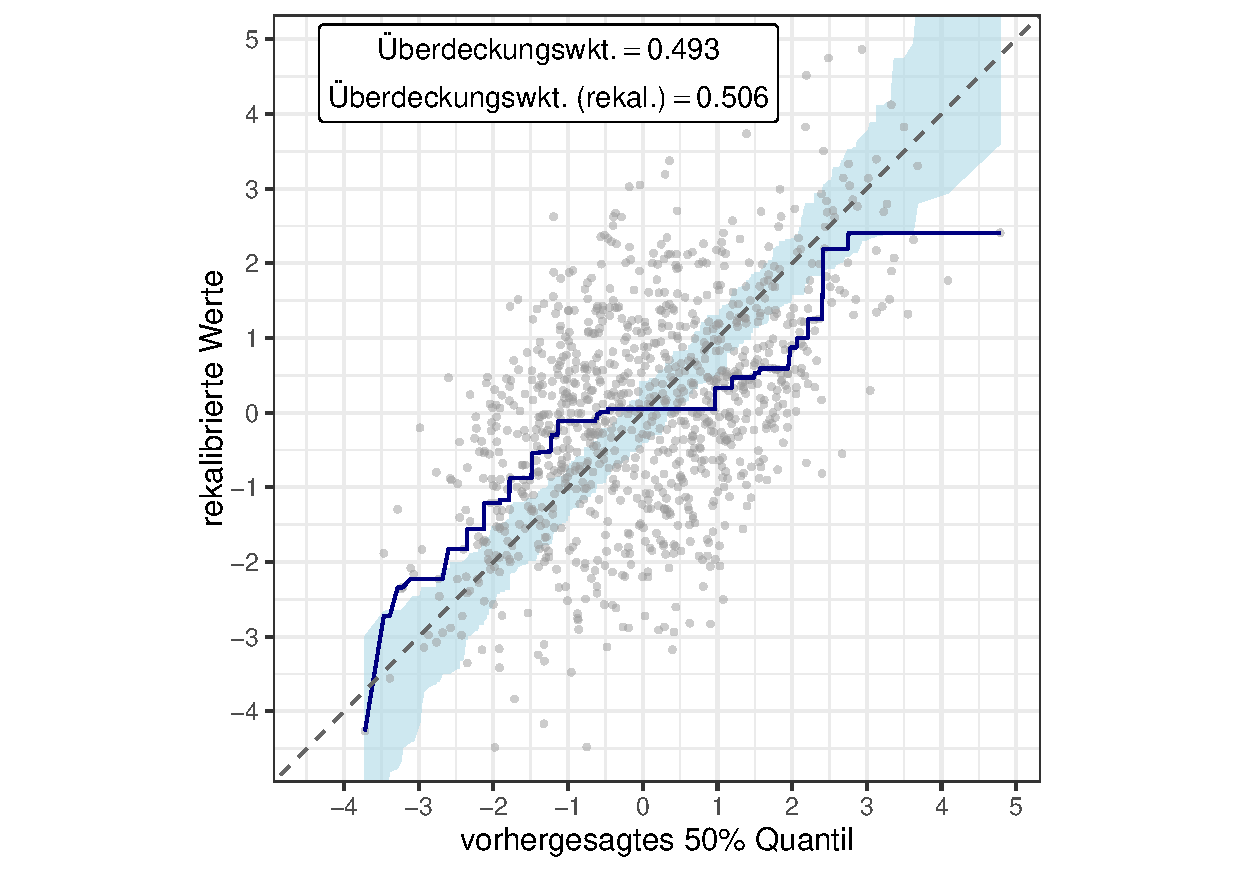
\includegraphics[width=0.7\linewidth]{figs/quant_cal.pdf}
    \caption{
    Empirisches Reliabilitätsdiagramm gemäß CORP-Ansatz für Beispiel \ref{bsp:quant_cal}. Hellblaue Bereiche entsprechen dem $95\%$-Konsistenzband basierend auf $100$ Replikationen. Punkte stellen Vorhersage-Beobachtungspaare dar.
    }
    \label{fig:quant_cal}
\end{figure}{}

Wieder können wir approzimativ Konsistenzbänder definieren unter Voraussetzung von Quantilkalibrierung. Das Verfahren ist beschrieben in \ref{sec:consistent_quant}.

Zusammenfassen können wir den CORP-Ansatz indem wir das Akronym entschlüsseln. CORP steht für Konsistent unter Annahme von Monotonie, optimally binned, reproduzierbar and PAV-based \parencite{gneiting2023regression,gneiting2023model}. PAV-based beschreibt die Methode, mit der die rekalibrierten Werte geschätzt werden, den Pool-adjacent-violator Algorithmus. Konsistent unter Monotonie, bedeutet, dass unter gültigen Voraussetzung der Monotonie das empirische Reliabilitätsdiagramm \eqref{eq:emp_rediag} ein konsistenter Schätzer für das Reliabilitätsdiagramm \eqref{eq:rediag} ist. Optimally binned, bedeutet, dass die erzeugten Bins unter den Voraussetzungen optimal bzgl. konsistenter Scoring-Functions sind, auf diese wir im Kapitel \ref{chap:scoring} näher eingehen. Reproduzierbarkeit bedeutet in diesem Zusammenhang, dass keine speziellen Hyperparameter oder Bin-Größen festgelegt werden müssen oder können, wodurch die Ergebnisse nachvollziehbar und wiederholbar bleiben.

Bislang haben wir immer \textit{ein} festes $\alpha$ betrachtet. Um Quantikalibrierung insgesamt gemäß \ref{def:all_quantcal} zu überprüfen, erstellen wir empirische Reliabilitätsdiagramme für eine ausgewählte Anzahl verschiedener  Quantileniveaus. Üblich sind die $25\%, 50\%, 75\%$ Quantile \parencite{gneiting2023model}.


\chapter{Zusammenhänge zwischen den Kalibrierungsbegriffen} \label{chap:cal_relation}
Im Folgenden beschreiben wir ausgewählte Zusammenhänge zwischen den verschiedenen Kalibrierungsbegriffen. Für eine ausführliche Aufschlüsselung der Zusammenhänge verschiedener Kalibrierungsbegriffe sei hier an \textcite{gneiting2023regression} verwiesen.

\begin{theo}[Auto-Kalibrierung impliziert marginale und probabilistische Kalibrierung \texorpdfstring{\parencite[Theorem 2.11]{gneitingCombining2013}})] \label{theo::AKthenPKMK}
Sei $F$ eine auto-kalibrierte Vorhersage bzgl. $Y$. Dann ist $F$ marginal und probabilistisch kalibriert bzgl. $Y$.
\end{theo}{}

Marginale und probabilistische Kalibrierung sind somit notwendig, aber nicht hinreichend für Auto-Kalibrierung. Auch wenn sie gemeinsam vorliegen, implizieren sie keine Auto-Kalibrierung \parencite[Example 2.4]{gneiting2023regression}.  Auch erfassen sie unterschiedliche Aspekte. So gibt es Vorhersagen, die marginal, aber nicht probabilistisch kalibriert sind sowie umgekehrt (siehe Beispiel \ref{bsp:kalunfoc}). Praktisch bedeutet es, dass wir zur Evaluation von Vorhersagen beide Kalibrierungsbedingungen überprüfen sollten.

\begin{theo}[Auto-Kalibrierung impliziert bedingte Quantilkalibrierung] \label{theo::AKthenTK}
Sei $F$ eine autokalibrierte Vorhersage bzgl. $Y$. Dann ist $F$ $\alpha$-quantilkalibriert bzgl. $Y$ für alle $\alpha \in (0,1)$
\end{theo}{}

Diese Aussage folgt aus Theorem 2.11 zusammen mit Propositon 2.18  von \textcite{gneiting2023regression} angewendet auf Quantile. Sie zeigen, dass Auto-Kalibrierung bedingte Kalibrierung für eine ganze Klasse statistischer Funktionale (Momente, Schwellenwerte, Quantile) impliziert.  Diese Klasse umfasst Funktionale, die durch sogenannte identifizierende Funktionen charakterisiert werden können.

Theorem \ref{theo::AKthenTK} und Theorem \ref{theo::AKthenPKMK} verdeutlichen, das die Auto-Kalibrierung die theoretisch stärkste Kalibrierungsbedingung ist. Die anderen Kalibrierungsbegriffe beschreiben daher Eigenschaften, die von Auto-Kalibrierung garantiert werden und ermöglichen jedoch eine empirische Untersuchung von diesen Aspekten.

Wie in Abschnitt \ref{sec:def_prob} angedeutet, sind probabilistische und unbedingte Quantilkalibrierung eng miteinander verbunden.

\begin{theo}[Probabilistische Kalibrierung impliziert unbedingte Quantilkalibrierung   \texorpdfstring{\parencite[A.5]{gneiting2023regression}})]\label{theo:pK-unbQK}
Sei $F$ eine probabilistisch kalibrierte Vorhersage bzgl. $Y$, dann ist $F$ unbedingte quantilkalibriert für alle $\alpha \in (0,1)$ bzgl. $Y$ gemäß \eqref{eq:uncond_pm_quant_cal}.\\
Sind alle Vorhersageverteilungen aus $F$ stetig und streng monoton steigend (auf gemeinsamen Träger) gilt Äquivalenz.
\end{theo}{}

Probabilistischer Kalibrierung impliziert jedoch nicht bedingte Quantilkalibrierung. Das Beispiel \ref{bsp:quant_cal} ist probabilistisch, aber nicht bedingt quantilkalibriert \parencite[Example 2.10]{gneiting2023regression}. Für die praktische Anwendung ergeben sich daraus zwei Konsequenzen: Erstens muss nach Überprüfung probabilistischer Kalibrierung die unbedingte Quantilkalibrierung nicht zusätzlich untersucht werden. Zweitens sollte vor der Untersuchung der bedingten Quantilkalibrierung zunächst die probabilistischen Kalibrierung betrachtet werden, weil sie Aufschluss über die unbedingte Quantilkalibrierung gibt.

Zusammenfassend gibt Tabelle \ref{tab:sum_kal} einen Überblick über die Kalibrierungsbegriffe, die zur empirischen Überprüfung in der vorliegenden Arbeit verwendet werden sollen.

\begin{table}[ht]
\caption{Informationsgehalt der verschiedenen Kalibrierungsbegriffe.}
\fontsize{10}{12}\selectfont
\label{tab:sum_kal}
\centering
\begin{tabularx}{\textwidth}{lXX}
\toprule
Kalibrierungsbegriff & Geprüfte Eigenschaft & Aussage bei erfüllter Kalibrierung \\
\midrule
Marginale Kalibrierung \\ &
Übereinstimmung der gemittelten Vorhersage mit Beobachtungen &
Die Vorhersage reproduziert die Marginalverteilung des Vorhersagegegenstandes.\\
\addlinespace
Probabilistische Kalibrierung \\ &
Bewertung des Gesamtbilds der vorhergesagten Verteilungen. Globale Über- bzw. Unterdispersion und systematische Verzerrung werden erkannt. &
Keine globalen Verzerrungen (Dispersion, Bias). Vorhersageintervalle werden getroffen. (Unbedingte) Quantile werden richtig vorhergesagt.\\
\addlinespace
Bedingte $\alpha$-Quantilkalibrierung\\ ($\alpha=0.25,0.5,0.75$) & Korrektheit ausgewählter Quantile bedingt auf den vorhergesagten Quantilwert. Überprüfen systematischer Fehler z.B. bei hohen bzw. niedrigen Vorhersagen. &
Die überprüften Quantile werden bedingt der Vorhersagesituation richtig getroffen. \\
\bottomrule
\end{tabularx}

\label{tab:calibration_summary}
\end{table}





